% Main thesis source. References are maintained in thebibliography below.
% No external .bib file or BibTeX step is required.
\documentclass[11pt,a4paper]{article}
\usepackage[margin=0.9in]{geometry}
\usepackage{times}
\usepackage{graphicx}
\usepackage{booktabs}
\usepackage{tabularx}
\usepackage{amsmath,amssymb}
\usepackage{titlesec}
\usepackage{enumitem}
\usepackage{authblk}
\usepackage{microtype}
\usepackage{tikz}
\usepackage{float}
\usepackage{hyperref}
\usetikzlibrary{
    arrows.meta,
    positioning,
    shapes.geometric,
    shapes.misc,
    fit,
    backgrounds
}


\hypersetup{colorlinks=true, linkcolor=blue, urlcolor=blue, citecolor=blue}

\titlespacing*{\section}{0pt}{8pt}{4pt}
\titlespacing*{\subsection}{0pt}{6pt}{3pt}

\title{\textbf{Can AI Help Moderate Community Voice Platforms?\\
Designing and Evaluating a Virtual Moderator}}
\author[]{Abhijeet Malik}
\affil[]{Supervised by Dr. Vikram Kamath Cannanure}
\date{}

\begin{document}
\maketitle

\begin{abstract}
\noindent Community voice platforms in rural and resource-constrained regions rely on human content moderators to listen to phone-call questions, understand local context, link questions to expert answers, and escalate urgent messages \cite{khullar2021moderation}. These moderators are frequently overwhelmed: while most incoming messages are routine questions, serious issues such as mental health crises or health misinformation are often hidden among them, and moderators cannot listen to all messages in time. This thesis investigates whether small language models (SLMs) can assist such moderators by giving feedback on every message, connecting questions with expert answers, and identifying transcription or speech issues, so that the human moderator only needs to review the messages that require attention. We design and evaluate a \emph{Virtual Moderator} built on privacy-preserving, resource-constrained SLMs for a healthcare moderation setting. The work is structured around three research questions: (RQ1) developing and validating a Virtual Moderator against human expert consensus, (RQ2) using the validated Virtual Moderator to compare candidate SLMs for deployment, and (RQ3) analyzing how speech-based interactions influence model performance. Initial results show that small models in the 1B--4B parameter range achieve moderate agreement with human moderators, and error analysis on speech-based interactions reveals that misinterpretation and lack of answers are the leading causes of model failure.
\end{abstract}


% ======================================================================
% INTRODUCTION
% ======================================================================
\section{Introduction}
\label{sec:introduction}

Voice-based community platforms allow people to seek information and share
experiences through ordinary mobile phones. Using Interactive Voice Response
(IVR), callers can listen to recordings and contribute messages without a
smartphone or an Internet connection. This form of participation is
particularly relevant where literacy, connectivity, or access to digital
devices limits the use of text-based services~\cite{khullar2021moderation}.

\emph{Mobile Vaani}, operated by the Indian social enterprise Gram Vaani,
illustrates the moderation work behind such services. Moderators review
recordings for audio quality, relevance, and compliance with editorial
guidelines. Khullar et al.~\cite{khullar2021moderation} reported that, at the
time of their study, approximately fifteen full-time moderators supported more
than forty forums receiving about 1,000 recordings per day. They investigated
AI tools for filtering empty recordings, assisting transcription, and
extracting metadata, finding opportunities to reduce routine work while
retaining human judgement for more complex decisions.

Evaluating answers to health questions introduces a further challenge. A
response may be fluent and related to the topic while still containing
incorrect information, omitting important qualifications, or suggesting help
that the caller cannot access. Research on health-focused AI safeguards
highlights the need to assess risks specific to health information and
advice~\cite{hewitt2025health}. In the Hindi sexual-health and mental-health
interactions considered in this thesis, an evaluator must consider both what
an answer says and how well it addresses the caller's situation. A general
assessment of whether the text sounds plausible is therefore insufficient.

This thesis investigates a \emph{Virtual Moderator}: a language-model-based
evaluator that assigns quality scores to question--answer pairs. Its assessment
follows two dimensions in the expert moderation scheme: \emph{Accuracy},
covering factual correctness, completeness, and safety; and \emph{Context \&
Relevance}, covering clarity, responsiveness to the question, and suitability
for the user's setting. For example, advice that depends on reliable Internet
access may be difficult to act on for a caller using a basic phone. The central
research problem is whether a compact model can apply these criteria
consistently enough to provide useful support for human review.

The study uses datasets provided by Gram Vaani to develop and evaluate this
approach. Human expert annotations provide the reference for assessing model
judgements, while labels generated by a larger language model provide
additional supervision for adapting the selected student model. These two
sources of annotation serve different purposes: learning to reproduce the
teacher's labels must be assessed separately from agreement with human
experts. The intended outcome is an evaluator whose strengths and errors can
be examined before its scores are used to support moderation decisions.

\emph{Small language models} (SLMs) are the focus because the intended
deployment setting calls for manageable memory requirements, inference costs,
and response times. Local inference could also reduce the need to send user
interactions to an external service during moderation. These are motivations
for investigating compact models; their practical value depends on the
quality of the resulting judgements. The thesis therefore examines model
performance against human annotations alongside the requirements of the
intended application.

Voice interaction adds another source of uncertainty. A caller's intended
question may differ from the text received by an answer-generation system
because of transcription errors, incomplete speech, or ambiguous phrasing.
An answer may consequently address a different concern from the one the
caller expressed. The study therefore also examines failures in speech-based
interactions, connecting the evaluation of written question--answer pairs
with the conditions in which the service is intended to operate.

\subsection{Motivating Scenario}

Consider an illustrative moderator, Amina, reviewing a Hindi voice interaction.
A teenager describes distress about school, and the answer-generation system
recommends an online counselling appointment. The response may appear relevant,
but Amina must check whether it addresses the concern expressed, whether its
claims are accurate, and whether the suggested service is accessible to this
caller. If the transcription has omitted part of the question, she must also
consider whether the answer responds to the caller's intended meaning.

In the proposed workflow, the Virtual Moderator would provide an initial
assessment of the question--answer pair for Amina to inspect. Its scores could
help her identify responses requiring closer review, while she retains
responsibility for the moderation decision. The experiment evaluates the
quality of these scores against human annotations. Reductions in workload
and improvements in service delivery are potential benefits to investigate
in deployment, rather than outcomes established by label agreement alone.

\subsection{Research Questions}

Based on these challenges, this thesis addresses the following research
questions:

\begin{itemize}[nosep]
    \item \textbf{RQ1:} How can a Virtual Moderator be developed and validated to evaluate responses in a healthcare context?

    \item \textbf{RQ2:} How do different AI models compare when evaluated using the Virtual Moderator developed in RQ1?

    \item \textbf{RQ3:} How do speech-based interactions influence AI model performance, and what opportunities and challenges emerge in the target context?
\end{itemize}

These questions organise the study around three intended contributions:
an evaluation of how closely a compact Virtual Moderator agrees with human
experts, a comparison of candidate answer-generation models using that
moderator, and an analysis of errors arising in speech-based interactions.
Using the moderator for model comparison requires establishing its reliability
and accounting for its limitations. Together, the analyses examine where
automated scoring can assist human moderation and where further review remains
necessary.

% ======================================================================
% RELATED WORK
% ======================================================================
\section{Related Work}
\label{sec:related-work}


The growing deployment of large language models (LLMs) in conversational systems has increased the need for reliable mechanisms that can detect harmful prompts, unsafe model responses, policy violations, and inappropriate refusals. Earlier content-moderation systems were commonly developed as task-specific classifiers for categories such as toxicity, hate speech, harassment, and sexually explicit content. However, the open-ended nature of LLM interactions introduces more complex risks, including harmful instructions, jailbreak attempts, context-dependent abuse, medical misinformation, and unsafe responses that may not contain explicitly toxic language. Consequently, recent research has shifted toward dedicated guard models, multilingual safety datasets, domain-specific risk taxonomies, and LLM-based evaluators. This section reviews these developments, with particular attention to efficient small language models, multilingual moderation, health-related risk detection, and the reliability of automated evaluation.

\subsection{LLM-Based Content Moderation and Guard Models}
One of the foundational works in modern LLM safeguarding is Llama Guard, introduced by \textbf{Inan et al.} \cite{inan2023llamaguard}. Unlike conventional toxicity classifiers that assign labels based on a fixed dataset, Llama Guard treats moderation as an instruction-following task governed by a configurable safety taxonomy. It can classify both user prompts and model-generated responses, thereby supporting input and output moderation within conversational applications. This policy-conditioned approach is important because the definition of unsafe content may vary across applications, organisations, and deployment contexts.
Subsequent guard models expanded the range of safety-related tasks. \textbf{WildGuard} \cite{han2024wildguard} provides a unified framework for identifying harmful user intentions, detecting harmful model responses, and determining whether a model has refused to answer. Its associated dataset includes direct and adversarial interactions across 13 risk categories. WildGuard is therefore relevant not only as a moderation model but also as an automated evaluator for safety-alignment experiments. In particular, its explicit treatment of refusal behaviour helps distinguish between unsafe compliance and appropriate rejection of harmful requests.
Similarly, \textbf{ShieldGemma} \cite{zeng2024shieldgemma} presents a family of content-moderation models based on Gemma 2. The models evaluate prompts and responses against safety policies related to sexually explicit material, dangerous content, harassment, and hate speech. ShieldGemma demonstrates the increasing use of generative, instruction-tuned models as policy-aware safety classifiers rather than relying exclusively on traditional encoder-based architectures. However, its core policies remain relatively broad and may not capture domain-specific harms, such as subtle medical misinformation or unsafe clinical recommendations.
Taxonomy design has also become a central component of guardrail development. \textbf{AEGIS2.0} \cite{ghosh2025aegis} introduces an adaptable safety taxonomy consisting of broad hazard categories and more fine-grained subcategories. It combines human annotation with judgments produced by multiple LLMs to construct a dataset of human–LLM interactions for guardrail development. This approach demonstrates that safety moderation cannot be reduced to a universal binary distinction between safe and unsafe content. Instead, useful moderation systems require explicit definitions of risks and sufficient flexibility to support different policies and application domains.
Collectively, these studies represent a transition from narrow toxicity detection toward general-purpose conversational safeguards. Nevertheless, general guard models introduce practical limitations. Their broad taxonomies may not represent risks that are specific to a particular domain, while the computational requirements of large generative guards can restrict their use in real-time, privacy-sensitive, or resource-constrained environments.


\subsection{Small Language Models for Efficient Moderation}
Although large guard models offer strong general-language capabilities, their inference costs, memory requirements, latency, and dependence on external services may make them unsuitable for some moderation applications. These limitations have motivated research into small language models (SLMs) that can be fine-tuned for specialised safety-classification tasks.
Zhan et al. introduced \textbf{SLM-Mod} \cite{zhan2024slmmod} to investigate whether specialised SLMs can provide an effective alternative to substantially larger LLMs for community-specific content moderation. The authors fine-tuned models with fewer than 15 billion parameters using approximately 150,000 comments collected from 15 Reddit communities. Their experiments showed that the fine-tuned SLMs outperformed zero-shot LLMs by an average of 11.5 percentage points in accuracy and 25.7 percentage points in recall. Few-shot prompting produced only limited improvements for the larger models. These findings suggest that task-specific supervision may be more important than model scale for well-defined moderation tasks.
SLM-Mod also demonstrates the importance of contextualising moderation policies. Content that is acceptable in one online community may violate the rules or expectations of another. Fine-tuned SLMs can learn such local distinctions while avoiding the expense of repeatedly querying a general-purpose LLM. However, the study is primarily concerned with Reddit community moderation. Social-media moderation differs from safety detection in health-related conversations, where risks may arise from inaccurate medical recommendations, delayed treatment, unsuitable medication guidance, failure to recognise emergencies, or inappropriate handling of sensitive personal information.
\textbf{Hewitt et al.} \cite{hewitt2025health} extend the SLM-based moderation problem into the healthcare domain by proposing a health-focused AI risk taxonomy developed through a literature review and co-design with healthcare professionals. The authors evaluate six SLMs using their proposed taxonomy and other safety taxonomies. Their findings show that Granite Guardian, an eight-billion-parameter model, was able to adapt to the health-focused taxonomy without additional fine-tuning and obtained an accuracy of 75\%. This result provides evidence that compact models can support domain-specific safety detection and may be suitable for local deployment in settings where privacy and computational efficiency are important.
These studies indicate that smaller, specialised models can be competitive with larger general-purpose models when the target risks and moderation policies are clearly defined. However, further investigation is required to determine whether these advantages generalise across languages, health-risk categories, prompt styles, and datasets that differ from the model’s training distribution.


\subsection{Parameter-Efficient Adaptation with LoRA and QLoRA}

Fine-tuning an entire language model can require substantial GPU memory and
computational resources, even when the target task is relatively specialised.
Hu et al.~\cite{hu2021lora} introduced Low-Rank Adaptation (LoRA) as a
parameter-efficient alternative to full fine-tuning. Instead of updating all
parameters of the pretrained model, LoRA keeps the original model weights
frozen and introduces small trainable low-rank matrices into selected
Transformer layers.

\subsubsection{Mathematical Formulation of LoRA}

Consider a pretrained linear transformation with weight matrix

\[
    \mathbf{W}_0 \in \mathbb{R}^{d \times k},
\]

where $\mathbf{W}_0$ represents the original pretrained weights. Under
conventional full fine-tuning, the complete matrix would be updated during
training,

\[
    \mathbf{W} = \mathbf{W}_0 + \Delta \mathbf{W},
\]

where $\Delta\mathbf{W}$ has the same dimensionality as
$\mathbf{W}_0$ and therefore contains $dk$ trainable parameters.

LoRA assumes that the task-specific weight update can be represented by a
matrix of substantially lower rank. Instead of directly learning
$\Delta\mathbf{W}$, it is decomposed as

\[
    \Delta\mathbf{W} = \mathbf{B}\mathbf{A},
\]

with

\[
    \mathbf{A} \in \mathbb{R}^{r \times k},
    \qquad
    \mathbf{B} \in \mathbb{R}^{d \times r},
\]

where

\[
    r \ll \min(d,k)
\]

is the LoRA rank. The effective weight matrix during inference is therefore

\[
    \mathbf{W}
    =
    \mathbf{W}_0
    +
    \mathbf{B}\mathbf{A}.
\]

For an input representation $\mathbf{x}$, the corresponding transformation
becomes

\[
    \mathbf{h}
    =
    \mathbf{W}_0\mathbf{x}
    +
    \mathbf{B}\mathbf{A}\mathbf{x}.
\]

In practice, LoRA introduces an additional scaling parameter $\alpha$, giving

\[
    \mathbf{h}
    =
    \mathbf{W}_0\mathbf{x}
    +
    \frac{\alpha}{r}
    \mathbf{B}\mathbf{A}\mathbf{x}.
\]

Here, $\mathbf{W}_0$ remains frozen throughout training, while only
$\mathbf{A}$ and $\mathbf{B}$ are updated by gradient descent.

The reduction in the number of trainable parameters can be seen directly.
Full fine-tuning of the original matrix requires

\[
    N_{\text{full}} = dk
\]

trainable parameters, whereas LoRA requires only

\[
    N_{\text{LoRA}}
    =
    r(k+d).
\]

The ratio of trainable LoRA parameters to full parameters is therefore

\[
    \frac{N_{\text{LoRA}}}{N_{\text{full}}}
    =
    \frac{r(k+d)}{dk}.
\]

Because $r$ is typically much smaller than either $d$ or $k$, only a small
fraction of the parameters of the original transformation need to be
optimised.

For example, if

\[
    d = k = 4096
\]

and a LoRA rank of

\[
    r = 16
\]

is used, full fine-tuning of the matrix would require

\[
    4096 \times 4096
    =
    16{,}777{,}216
\]

trainable parameters. In contrast, LoRA requires only

\[
    16(4096 + 4096)
    =
    131{,}072
\]

trainable parameters for the corresponding update. This is less than
one percent of the parameters required to update the complete matrix.

In Transformer-based language models, LoRA is commonly applied to the
projection matrices used in the attention mechanism. In this work, adapters
are introduced into the query, key, value, and output projections,

\[
    \mathbf{W}_{Q},\;
    \mathbf{W}_{K},\;
    \mathbf{W}_{V},\;
    \mathbf{W}_{O},
\]

while the original pretrained parameters remain fixed. For example, the
query projection becomes

\[
    \mathbf{W}_{Q}^{\prime}
    =
    \mathbf{W}_{Q}
    +
    \frac{\alpha}{r}
    \mathbf{B}_{Q}\mathbf{A}_{Q}.
\]

The same principle is applied independently to the other selected projection
matrices.

\subsubsection{QLoRA}

Dettmers et al.~\cite{dettmers2023qlora} extended this approach with Quantized Low-Rank
Adaptation (QLoRA). QLoRA further reduces memory consumption by storing the
frozen pretrained model in a low-precision quantized representation while
keeping the LoRA adapters trainable.

Let

\[
    Q(\mathbf{W}_0)
\]

denote the quantized representation of the pretrained weight matrix.
During computation, the quantized weights are interpreted using an
appropriate dequantization operation,

\[
    \widetilde{\mathbf{W}}_0
    =
    Q^{-1}\bigl(Q(\mathbf{W}_0)\bigr).
\]

The adapted transformation can then be expressed as

\[
    \mathbf{h}
    =
    \widetilde{\mathbf{W}}_0\mathbf{x}
    +
    \frac{\alpha}{r}
    \mathbf{B}\mathbf{A}\mathbf{x}.
\]

The quantized base-model parameters remain frozen. Gradients are propagated
through the model in order to optimise only the LoRA matrices
$\mathbf{A}$ and $\mathbf{B}$:

\[
    \nabla_{\mathbf{W}_0}\mathcal{L} = 0,
\]

while

\[
    \nabla_{\mathbf{A}}\mathcal{L} \neq 0,
    \qquad
    \nabla_{\mathbf{B}}\mathcal{L} \neq 0.
\]

Thus, the optimisation problem can be written conceptually as

\[
    \mathbf{A}^{*},\mathbf{B}^{*}
    =
    \arg\min_{\mathbf{A},\mathbf{B}}
    \mathcal{L}
    \left(
        f_{\mathbf{W}_0,\mathbf{A},\mathbf{B}}(x),
        y
    \right),
\]

where $x$ denotes the moderation input, $y$ denotes the target moderation
labels, and $\mathcal{L}$ is the training loss.

For the Virtual Moderator, the target $y$ consists of the two
teacher-generated moderation decisions,

\[
    y =
    \left(
        y_{\text{Accuracy}},
        y_{\text{Context\&Relevance}}
    \right),
\]

with

\[
    y_{\text{Accuracy}},
    y_{\text{Context\&Relevance}}
    \in \{0,1,2\}.
\]

Consequently, the pretrained language model provides the underlying linguistic
and reasoning capabilities, while the LoRA adapters learn the task-specific
mapping from a healthcare question--answer pair to the required moderation
labels.

% TODO: This describes a previous configuration. The reviewed notebook uses
% unquantized BF16, r=8, alpha=16, and Accuracy-only targets. Attribute
% configurations to specific runs before presenting one as the final method.
In the implementation used in this work, the base language model is loaded
using 4-bit quantization and LoRA adapters are trained on selected attention
projection layers. A rank of $r=16$ and scaling factor $\alpha=32$ are used.
The resulting architecture can be summarised as

\[
    \boxed{
    \text{Frozen 4-bit Base Model}
    +
    \text{Trainable LoRA Adapters}
    }
\]

rather than updating the complete multi-billion-parameter model.

This formulation is particularly suitable for the iterative supervision
pipeline used in this thesis. At each training-set size, the same pretrained
base model can be retained while a lightweight LoRA adapter is learned from
the available Claude-generated supervision. This makes it possible to compare
adaptation with increasing numbers of labelled examples without repeatedly
performing computationally expensive full-model fine-tuning.


\subsection{Multilingual and Culturally Grounded Safety Moderation}
A significant limitation of existing safety research is its concentration on English-language data. Safety alignment learned predominantly from English examples may not transfer consistently to other languages, particularly languages with fewer training resources or different cultural expressions of harmful content.
Wang et al. introduced \textbf{XSafety} \cite{wang2024languages}, one of the earliest systematic multilingual safety benchmarks for LLMs. XSafety covers 14 safety scenarios across ten languages, including Hindi. The evaluation demonstrated that the tested LLMs generated substantially more unsafe responses for non-English prompts than for equivalent English prompts. This finding indicates that general multilingual capability does not necessarily imply multilingual safety and that safety alignment can weaken when interactions are conducted in languages that are less represented in training data.
The distinction between linguistic translation and cultural adaptation is further examined in \textbf{RTP-LX} \cite{dewynter2024rtplx}. RTP-LX contains human-transcreated and human-annotated toxic prompts and outputs in 28 languages. Instead of depending entirely on literal machine translation, the dataset uses participatory design and includes culturally specific forms of toxicity. Its evaluation shows that models may achieve apparently acceptable accuracy while still exhibiting weak agreement with human judgments, particularly for context-dependent harms, microaggressions, and subtle bias. The work therefore highlights the importance of considering annotation agreement and class distribution rather than relying only on aggregate accuracy.
Building on multilingual safety datasets, Kumar et al. proposed \textbf{PolyGuard} \cite{kumar2025polyguard}, a multilingual safety-moderation model covering 17 languages, including Hindi. PolyGuard is trained on PolyGuardMix, which contains approximately 1.91 million multilingual examples. The authors also introduce PolyGuardPrompts, an evaluation benchmark containing approximately 29,000 samples. The datasets label prompt harmfulness, response harmfulness, and response refusal, allowing PolyGuard to address a set of moderation tasks similar to WildGuard in a multilingual setting. PolyGuard reportedly improves over existing open and commercial safety classifiers across several safety and toxicity evaluations.
PolyGuard represents an important step toward scalable multilingual moderation. Nevertheless, part of its data is produced through human-verified machine translation of English safety examples. Translation-based scaling improves language coverage, but translated examples may preserve the assumptions and risk definitions of the source language. They may fail to capture native expressions, code-switching, region-specific medical practices, culturally sensitive health topics, or harmful content that depends on local social context. Multilingual moderation should therefore be evaluated not only on translated test sets but also on naturally occurring and culturally grounded examples.
Overall, multilingual safety research shows that performance can vary considerably across languages even when the underlying harmful intent is equivalent. It also suggests that low-resource and culturally diverse languages require language-aware evaluation rather than being treated as direct translations of English.


\subsection{Safety Benchmarks and Domain-Specific Risk Taxonomies}
The reliability of a moderation model depends heavily on the datasets and taxonomies used to train and evaluate it. Many earlier toxicity benchmarks were constructed from social-media posts and comments. However, user interactions with conversational AI systems differ from conventional social-media communication in their structure, purpose, and context.
\textbf{ToxicChat} \cite{lin2023toxicchat} addresses this limitation by introducing a benchmark derived from real user queries submitted to an open-source chatbot. The dataset contains approximately 10,000 user–AI conversations and includes nuanced examples that are difficult for models trained on conventional social-media toxicity datasets. Experiments reported in the study reveal a meaningful domain shift between social-media toxicity detection and moderation of user–AI interactions. This finding supports the use of conversational data when evaluating guard models intended for chatbot deployment.
Broader evaluation frameworks have also attempted to organise safety risks systematically. \textbf{SALAD-Bench} \cite{li2024saladbench} introduces a large-scale benchmark with a three-level hierarchical taxonomy. It includes conventional safety questions as well as examples modified using adversarial attacks and defence strategies. SALAD-Bench also proposes MD-Judge, an LLM-based evaluator that assesses question–answer pairs according to multiple safety dimensions. The hierarchical structure is useful because it enables performance to be examined at different levels of granularity rather than reporting only an overall safe-versus-unsafe score.
General safety taxonomies, however, may not sufficiently represent risks encountered in healthcare applications. A health-related response can be harmful without containing hate speech, violence, explicit content, or illegal instructions. Examples include confidently presenting incorrect medical information, recommending an unsuitable treatment, failing to advise emergency assistance, contradicting established clinical evidence, or encouraging a user to discontinue prescribed medication.
\textbf{MedSafetyBench} \cite{han2024medsafetybench} addresses this problem by defining medical safety with reference to principles of medical ethics and constructing a benchmark for evaluating medical LLMs. Its evaluation indicates that strong performance on medical question-answering tasks does not guarantee safe behaviour. The study also shows that safety-oriented fine-tuning can improve medical safety while retaining general medical performance. MedSafetyBench and the health-focused taxonomy proposed by \textbf{Hewitt et al.} \cite{hewitt2025health} therefore complement general guardrail taxonomies by demonstrating that safety definitions should account for the requirements of the target domain.
An additional challenge in health-related moderation is avoiding excessive blocking. Terms related to suicide, substance use, medication, abuse, sexual health, or serious illness may occur in legitimate requests for information or assistance. A moderator that relies primarily on the presence of sensitive vocabulary may incorrectly classify beneficial health conversations as unsafe. Consequently, a suitable health-moderation system must balance the recall of genuinely harmful content against the false-positive classification of legitimate, educational, or help-seeking content.


\subsection{LLMs as Automated Judges}
Human evaluation is often considered the most reliable method for assessing open-ended language-model outputs, but it is expensive, time-consuming, and difficult to scale. LLM-as-a-judge methods have therefore become increasingly common in model evaluation.
\textbf{Zheng et al.} \cite{zheng2023judging} introduced MT-Bench and Chatbot Arena to investigate whether strong LLMs could approximate human preferences when comparing chatbot responses. Their results showed that an LLM judge could achieve more than 80\% agreement with human preferences. The study also identified important limitations, including position bias, verbosity bias, self-enhancement bias, and limited reasoning ability. These observations established both the potential and the risks of using LLMs as automatic evaluators.
Later work has examined the reliability of judge models more directly. \textbf{JudgeBench} \cite{tan2024judgebench} evaluates LLM judges using difficult response pairs from knowledge, reasoning, mathematics, and programming tasks where preference labels are based on more objective correctness criteria. The benchmark shows that several otherwise capable models struggle to distinguish between subtly different responses. This suggests that agreement with general human preference does not necessarily establish the reliability of a judge for specialised evaluation tasks.
Safety evaluation presents additional difficulties because judgments may depend on policy interpretation and contextual reasoning. Chen and \textbf{Goldfarb-Tarrant} \cite{chen2025safer} evaluate 11 LLM judges across safety domains and examine their self-consistency, agreement with human annotations, and sensitivity to superficial response features. Their results show that safety judgments can be influenced by artefacts such as apologetic phrasing and response verbosity. A response may therefore appear safer to an automated evaluator because it uses cautious language, even when its substantive content remains harmful.
The reliability problem becomes especially important in the medical domain. \textbf{Diekmann et al.} \cite{diekmann2025medicaljudges} compare LLM-based medical safety judgments with human annotations across several qualitative criteria. Although the evaluated judges perform comparatively well on more objective properties, such as grammaticality and consistency with established scientific knowledge, they experience greater difficulty with subjective and context-dependent safety dimensions. This result supports the use of expert or human-validated annotations when assessing health-related moderation systems.
LLM judges remain useful for scalable experimentation, particularly when comparing many model configurations. However, their outputs should not automatically be treated as ground truth. Robust evaluation practices may include the use of explicit rubrics, randomisation of response order, repeated evaluations, multiple judges, reporting of inter-rater agreement, and validation against a human-annotated subset.


\subsection{Summary and Research Gap}
Existing research has made substantial progress in developing general-purpose guard models, efficient SLM-based classifiers, multilingual safety benchmarks, domain-specific risk taxonomies, and scalable LLM-based evaluation. Nevertheless, these research directions have often been examined separately.
General-purpose safeguards such as Llama Guard, WildGuard, ShieldGemma, and AEGIS2.0 provide broad coverage of conversational risks but are not specifically designed to distinguish between safe and unsafe health-related communication. Research on SLMs demonstrates that specialised compact models can outperform much larger zero-shot models, although much of this evidence is based on social-media or community-moderation data. Health-safety benchmarks and taxonomies capture domain-specific risks, but multilingual variation and deployment efficiency remain comparatively underexplored. Multilingual systems such as PolyGuard improve cross-lingual coverage, yet multilingual safety data continue to depend partly on translated English examples and may not adequately represent culturally grounded health risks. Finally, LLM-based judges provide scalable evaluation but may introduce inconsistent or artefact-sensitive judgments.
These limitations motivate research at the intersection of efficient SLM-based moderation, multilingual safety, health-focused risk classification, and reliable evaluation. In particular, there remains a need to determine whether compact language models can identify fine-grained health-related risks across languages such as English and Hindi while maintaining a suitable balance between harmful-content detection and the preservation of legitimate health discussions. Such evaluation should consider not only overall accuracy but also class-specific precision, recall, F1-score, false-positive behaviour, cross-language generalisation, and agreement with human or expert judgments. This combined perspective can support the development of moderation systems that are computationally efficient, context-sensitive, linguistically inclusive, and appropriate for safety-critical health applications.


% ======================================================================
% DATASET
% ======================================================================
\section{Dataset}
\label{sec:dataset}
All the following datadset are made available by Gram Vaani . These are all the real question answers asked by Users in the region . These questions are being fed to the Knowledge based model , Sarvam AI. The answers  generated are being reported as answer . we have the sanitized version of the Queries and also the original question asked by the Users . There is no sanitized data used in the making of the Virtual Moderator .  
Three distinct datasets support the three research questions of this thesis.

\subsection{RQ1 Dataset}
% TODO: Reconcile the stated 1,660/150 counts with the inspected local
% files (1,658 source rows; 166 rows in final_test.xlsx). Confirm split
% membership and prior training exposure before claiming an untouched test set.
% Current plan: finish Claude annotation of the corpus before new experiments;
% revise the historical batch-wise annotation description once the protocol is fixed.
For the initial validation and benchmarking of the Virtual Moderator, a fixed
human-annotated healthcare moderation dataset of 100 question--answer pairs is
used. Each instance is labelled by human moderators for two dimensions:
\emph{Accuracy} and \emph{Context \& Relevance}, both on a three-level scale
from 0 to 2. This 100-example dataset is retained as the fixed validation set
throughout the subsequent adaptation experiments and is never used for LoRA
parameter updates.

A larger pool of 1{,}660 previously unlabelled question--answer pairs is
available for iterative adaptation. It contains 296 mental-health queries and
1{,}364 sexual-health queries. Before adaptation begins, 150 examples are
separated using a stratified shuffle procedure and reserved as a final
held-out test set. These examples are not used for prompt optimization,
training, model selection, or intermediate error analysis.

The remaining examples form the iterative supervision pool. Successive batches
of 100 examples are labelled by a Claude-based external teacher model using
the same Accuracy and Context \& Relevance rubric. These teacher-generated
labels are treated as pseudo-labels for prompt optimization and LoRA/QLoRA
instruction fine-tuning of the selected student model.

\subsection{RQ2 Dataset}
RQ2 uses the larger healthcare question--answer collection to compare candidate
models at scale after the Virtual Moderator has been established. The dataset
contains naturally occurring Hindi user questions and the corresponding
answers produced in the target application setting, together with translated
versions where available. The original Hindi text is used for the moderation
experiments.

The dataset does not initially contain Accuracy or Context \& Relevance labels
for all examples. During RQ1 adaptation, labels for the training batches are
generated by the Claude teacher model. The fixed 100-example human-labelled
validation set and the 150-example held-out final test set remain separate from
these iterative training batches.

\subsection{RQ3 Dataset}
For analyzing speech-based interactions, a dataset of 140 queries collected from 10 users is used, with each user asking 14 questions to the model, including some repeated questions. This dataset enables both category-wise (mental health vs.\ sexual health) and user-wise error analysis.
This dataset also contains the labels for correct , incorrect and minor error for the answers generated by Sarvam AI . These labels are given by the Experts working for the NGO 

% ======================================================================
% METHODOLOGY
% ======================================================================
\section{Methodology}
\label{sec:methodology}

This section describes the construction and validation of the Virtual Moderator
in RQ1, the comparison of candidate models in RQ2, and the error analysis used
for speech-based interactions in RQ3. RQ1 consists of two stages: an initial
benchmark against human expert labels, followed by LLM-assisted iterative
supervision of selected resource-efficient models.

\subsection{RQ1: Building and Validating the Virtual Moderator}
\label{subsec:rq1}

RQ1 investigates whether a Small Language Model (SLM) can act as a
\emph{Virtual Moderator} whose decisions are sufficiently aligned with those
of human healthcare experts. The human-annotated healthcare moderation dataset
is used as the reference standard. Each data instance contains a Hindi user
question, its corresponding expert answer, and expert-assigned labels for two
moderation dimensions:

\begin{enumerate}[nosep]
    \item \textbf{Accuracy:} whether the answer is factually correct and
    appropriate for the healthcare question; and
    \item \textbf{Context and Relevance:} whether the answer addresses the
    user's question and is suitable within the context of the interaction.
    
\end{enumerate}          
Both dimensions are represented on the scale $\{0,1,2\}$, where 0 denotes
the lowest assessment, 1 denotes a partially satisfactory assessment, and 2
denotes the highest assessment.

The original Hindi questions and answers are used directly during inference.
They are not translated into English. This preserves the linguistic
characteristics of the original interactions, including informal expressions,
code-switching, regional vocabulary, and possible speech-transcription errors.

\subsubsection{Candidate Model Selection}

The candidate model set includes general-purpose language models,
healthcare-oriented models, safety and harm-detection models, and models
previously proposed for content-moderation tasks. Models available through the
Ollama ecosystem are included irrespective of model size, provided that they
can process the required context length.

Models with up to 8 billion parameters are downloaded and executed locally.
This allows their performance to be evaluated under the privacy and resource
constraints expected in the intended deployment environment. Models larger
than 8 billion parameters are executed using a cloud server because they
cannot be run reliably on the available local hardware. Where supported,
larger models are loaded using 4-bit quantization to reduce memory consumption
and inference cost.

\subsubsection{Inference Procedure}

Each model receives the Hindi question and its corresponding expert answer and
is instructed to predict the labels for Accuracy and Context and Relevance.
The question--answer pairs contain approximately 3,000 tokens in the largest
cases. To manage memory usage and inference time, the data are processed in
batches of 16 instances.

Each question--answer pair is evaluated  by every candidate model.
Repeated inference is used to measure the stability of the model's moderation
decision and to reduce the effect of stochastic generation. 

The models are instructed to return only a predefined JSON object and no
additional explanation. A simplified output format is shown below:

\begin{verbatim}
{
  "accuracy": 1,
  "context_relevance": 1
}
\end{verbatim}

All generated outputs are parsed automatically. An output is considered valid
only when it:

\begin{enumerate}[nosep]
    \item can be parsed as JSON;
    \item contains all required fields; and
    \item contains labels within the permitted numerical range.
\end{enumerate}

If the model returns malformed JSON, additional text that cannot be parsed, a
missing field, or no numerical label, the corresponding output is initially
stored as \texttt{None}. During preprocessing, these invalid outputs are
encoded as \texttt{-1}. The value \texttt{-1} is used only as an inference
failure indicator and is not interpreted as a valid moderation class.
JSON-format failure rates are reported separately. For end-to-end system
evaluation, invalid outputs are also counted as unsuccessful moderation
attempts.

\subsubsection{Evaluation Against Human Expert Consensus}

The labels generated by each model are compared with the labels assigned by
the project experts. Precision, recall, and F1-score are calculated separately
for Accuracy and Context and Relevance. Macro-averaged F1-score is used as the
primary comparison metric because it gives equal importance to all label
classes and is less affected by class imbalance than overall accuracy.

In addition to the class-level metrics, the following measures are reported:

\begin{enumerate}[nosep]
    \item agreement between the model and the expert reference labels;
    \item disagreement across the three repeated model runs;
    \item JSON-format and parsing failure rate;
    \item category-specific performance for mental-health and sexual-health
    questions; and
    \item local inference latency and memory consumption, where applicable.
\end{enumerate}

Candidate models are compared primarily using macro-F1 against the expert
labels, together with output stability and deployment cost. Because several
models obtain similar F1 scores despite large differences in parameter count,
model size and local deployment feasibility are also considered. Therefore,
resource-efficient models in the approximately 4B--8B range with competitive
validation performance are shortlisted for further adaptation rather than
selecting a substantially larger model solely for a small numerical gain.
\subsubsection{LLM-Assisted Iterative Supervision}
\label{subsec:llm_iterative_supervision}

After the initial benchmark, resource-efficient student models with competitive
macro-F1 scores are selected for adaptation. The refinement stage follows an
\emph{LLM-assisted iterative supervision} strategy. A stronger external
language model, Claude, acts as the teacher and generates pseudo-labels for
previously unlabelled examples, while the selected locally deployable model,
for example Gemma~3~4B, acts as the student.

The 100 human-labelled examples used during the initial benchmark are retained
as a fixed validation set. They are not used for LoRA training. Before the
iterative adaptation begins, 150 examples are also separated from the larger
unlabelled pool using stratified shuffling and stored as a final held-out test
set. This final test set is not used for prompt optimization, fine-tuning,
intermediate model selection, or error-driven decisions.

The iterative refinement procedure is performed as follows:

\begin{enumerate}[nosep]
    \item \textbf{Select a fresh batch:}
    A new batch of 100 previously unused question--answer pairs is sampled from
    the iterative training pool.

    \item \textbf{Teacher annotation:}
    Claude receives the question--answer pairs together with the predefined
    moderation rubric and assigns an Accuracy label and a Context \& Relevance
    label from $\{0,1,2\}$. These labels are treated as
    \emph{teacher-generated pseudo-labels}.

    \item \textbf{Prompt optimization:}
    During the first adaptation round, several moderation-prompt variants are
    evaluated against the Claude-generated labels. The prompt with the strongest
    macro-F1 is selected and then frozen so that later training rounds remain
    directly comparable.

    \item \textbf{Student prediction and error analysis:}
    The student model predicts the labels for the new batch without seeing the
    teacher labels. Its predictions are compared with Claude's labels. Errors
    may be grouped into categories such as confusion between neighbouring
    classes, context loss, overgeneralisation, or output-format failure.
    Importantly, the student's incorrect predictions are not used as training
    targets; the Claude-generated labels provide the supervision signal.

    \item \textbf{LoRA/QLoRA instruction fine-tuning:}
    Each example is converted into an instruction--response pair consisting of
    the frozen moderation prompt, the healthcare question and answer, and the
    Claude-generated target labels. The base-model weights remain frozen and
    only the LoRA adapter parameters are optimized.

    \item \textbf{Validation:}
    After fine-tuning, the adapted model is evaluated on the same fixed
    100-example human-labelled validation set. Accuracy macro-F1, Context \&
    Relevance macro-F1, and the aggregate score are recorded.

    \item \textbf{Cumulative expansion:}
    A further batch of 100 unused examples is labelled by Claude and added to
    the existing training data. Thus, the amount of supervision grows
    cumulatively:
    \[
        100 \rightarrow 200 \rightarrow 300 \rightarrow 400
        \rightarrow \cdots
    \]
    For each training-set size, the same frozen prompt and validation set are
    used. This produces a learning curve showing how much performance improves
    as additional teacher-labelled data are introduced.

    \item \textbf{Final model selection and testing:}
    After the prompt, model, and LoRA configuration have been finalized using
    validation performance, the selected configuration is evaluated on the
    untouched 150-example test set. This final evaluation provides the estimate
    of generalisation performance reported for the adapted Virtual Moderator.
\end{enumerate}

The procedure is therefore a teacher--student adaptation framework rather than
a conventional Human-in-the-Loop process. Human annotations establish the
fixed validation reference, whereas Claude provides the scalable supervision
used during iterative model adaptation. In this thesis, this process is
referred to as \emph{LLM-assisted iterative supervision}.

\begin{figure}[H]
\centering
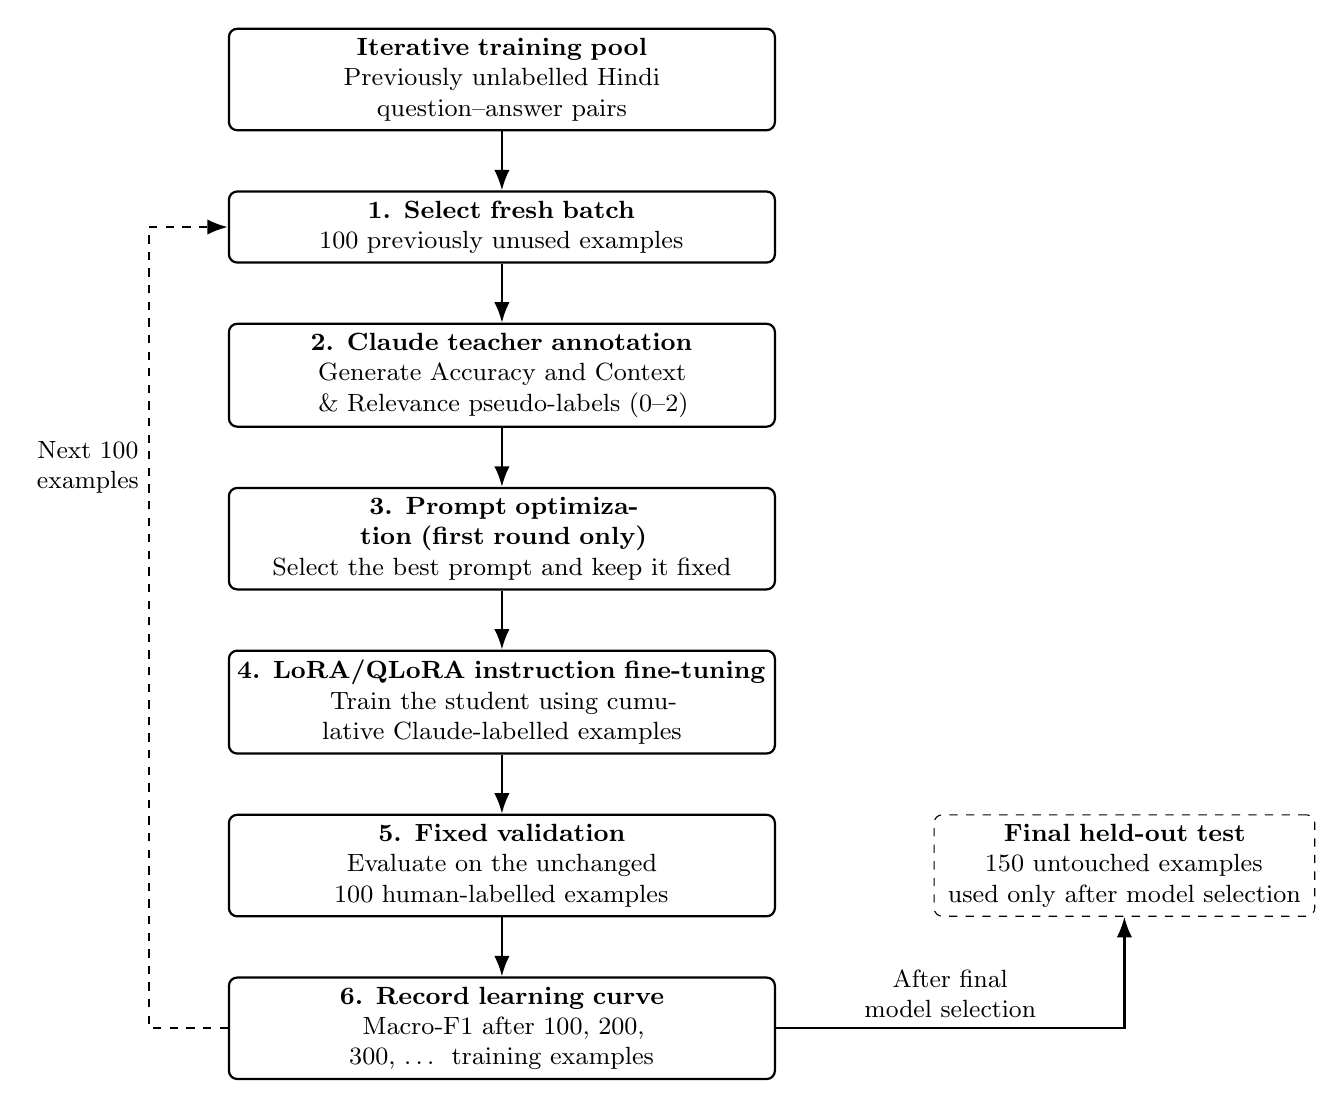
\begin{tikzpicture}[
    node distance=0.75cm,
    every node/.style={font=\small},
    flowbox/.style={
        rectangle,
        rounded corners=3pt,
        draw,
        thick,
        align=center,
        text width=6.7cm,
        minimum height=0.85cm
    },
    side/.style={
        rectangle,
        rounded corners=3pt,
        draw,
        dashed,
        align=center,
        text width=4.6cm,
        minimum height=0.85cm
    },
    arrow/.style={-{Latex[length=2.6mm]}, thick},
    loop/.style={-{Latex[length=2.6mm]}, thick, dashed}
]

\node[flowbox] (pool)
{\textbf{Iterative training pool}\\Previously unlabelled Hindi question--answer pairs};

\node[flowbox, below=of pool] (batch)
{\textbf{1. Select fresh batch}\\100 previously unused examples};

\node[flowbox, below=of batch] (claude)
{\textbf{2. Claude teacher annotation}\\Generate Accuracy and Context \& Relevance pseudo-labels (0--2)};

\node[flowbox, below=of claude] (prompt)
{\textbf{3. Prompt optimization (first round only)}\\Select the best prompt and keep it fixed};

\node[flowbox, below=of prompt] (train)
{\textbf{4. LoRA/QLoRA instruction fine-tuning}\\Train the student using cumulative Claude-labelled examples};

\node[flowbox, below=of train] (validate)
{\textbf{5. Fixed validation}\\Evaluate on the unchanged 100 human-labelled examples};

\node[flowbox, below=of validate] (record)
{\textbf{6. Record learning curve}\\Macro-F1 after 100, 200, 300, \ldots{} training examples};

\node[side, right=2.0cm of validate] (test)
{\textbf{Final held-out test}\\150 untouched examples\\used only after model selection};

\draw[arrow] (pool) -- (batch);
\draw[arrow] (batch) -- (claude);
\draw[arrow] (claude) -- (prompt);
\draw[arrow] (prompt) -- (train);
\draw[arrow] (train) -- (validate);
\draw[arrow] (validate) -- (record);

\draw[loop]
    (record.west)
    -- ++(-1.0,0)
    |- node[pos=0.35, left, align=center]
       {Next 100\\examples}
    (batch.west);

\draw[arrow]
    (record.east)
    -| node[pos=0.25, above, align=center]
       {After final\\model selection}
    (test.south);

\end{tikzpicture}

\caption{LLM-assisted iterative supervision pipeline. Claude provides
pseudo-labels for successive batches of previously unlabelled examples. The
student model is adapted using a fixed optimized prompt and LoRA/QLoRA, while
performance is measured after each round on the same 100-example human-labelled
validation set. The 150-example final test set remains untouched until the
model configuration is finalized.}
\label{fig:llm-assisted-iterative-supervision}
\end{figure}

\subsection{RQ2: Comparing Candidate SLMs Using the Virtual Moderator}
\label{subsec:rq2}

After the Virtual Moderator has been validated against human expert consensus,
it is used to compare candidate SLMs that could generate answers for the
community voice platform. This stage separates the model that \emph{evaluates}
answers from the candidate models that \emph{generate} them.

The comparison is conducted in four steps:

\begin{enumerate}[nosep]
    \item \textbf{Response Generation:}
    Each healthcare question is provided to every candidate SLM. The questions
    are processed in small batches, and each model generates an answer in the
    original language of the interaction.

    \item \textbf{Evaluation by the Virtual Moderator:}
    Each generated answer is paired with its original question and provided to
    the validated Virtual Moderator from RQ1. The Virtual Moderator assigns an
    Accuracy label and a Context \& Relevance label to the generated response.

    \item \textbf{Quality and Efficiency Comparison:}
    The candidate models are compared across two groups of criteria.
    \emph{Quality} is assessed using the Accuracy and Context and Relevance
    moderation results. \emph{Efficiency} is assessed using inference latency,
    peak memory consumption, model size, quantization level, and hardware
    requirements.

    \item \textbf{Candidate Selection:}
    The most suitable SLM is selected using a ranked comparison of quality and
    efficiency. The selected model is not necessarily the model with the
    highest quality score alone; preference is given to a model that provides
    an appropriate balance between response quality, privacy, latency, memory
    use, and feasibility of local deployment.
\end{enumerate}

The comparison therefore evaluates both whether a model can generate suitable
healthcare answers and whether it can operate under the computational
constraints of the target community platform.


\subsection{RQ3: Analysis of Speech-Based Interactions}
\label{subsec:rq3}

RQ3 examines how speech-based input affects the performance of the Virtual
Moderator. Community voice messages differ from carefully written text because
they may contain incomplete sentences, repetition, hesitation, background
noise, regional pronunciation, code-switching, ambiguous references, and
automatic speech-recognition errors. These characteristics may cause the model
to misunderstand the question even when the underlying healthcare concern is
valid and important.

The purpose of this analysis is to determine:

\begin{enumerate}[nosep]
    \item how the Virtual Moderator's errors are distributed;
    \item which types of failure account for the largest proportion of errors;
    \item whether mental-health or sexual-health questions produce more errors;
    \item whether particular users or speaking styles are associated with
    higher error rates; and
    \item how frequently errors originate from the speech or transcription
    rather than from the moderation model itself.
\end{enumerate}

The analysis is conducted in four stages.

\begin{enumerate}[nosep]
    \item \textbf{Outcome Classification:}
    Each moderation decision is classified as \emph{Correct},
    \emph{Minor Error}, or \emph{Incorrect}. A minor error is assigned when
    the model's decision is partially appropriate but differs from the expert
    label in a way that does not completely change the interpretation of the
    answer.

    \item \textbf{Error-Cause Annotation:}
    Every minor or incorrect prediction is assigned one or more error causes.
    The error taxonomy includes misinterpretation of the question, missing or
    insufficient answer content, irrelevant answer content, factual
    inaccuracy, loss of context, ambiguous speech, transcription error,
    code-switching, incomplete utterance, and output-format failure.

    \item \textbf{Health-Category Analysis:}
    Error rates are calculated separately for mental-health and sexual-health
    interactions. This analysis identifies whether one healthcare category
    presents greater difficulty for the Virtual Moderator and which error types
    are most frequent within each category.

    \item \textbf{User-Level Analysis:}
    Errors are grouped by user or speaker to determine whether performance is
    affected by individual speech characteristics. The analysis considers the
    number of messages contributed by each user, the frequency of errors, and
    the dominant error causes. Where available, transcript quality and
    speech-recognition errors are examined alongside the moderation results.
\end{enumerate}

The RQ3 analysis distinguishes between errors caused by the Virtual Moderator
and errors inherited from earlier stages of the speech-processing pipeline.
For example, a medically important term may be transcribed incorrectly, a
negation may be omitted, or the user's main question may be obscured by
disfluencies. In such cases, the moderation failure may originate from the
transcript rather than from the model's moderation capability.

The results are reported using overall error frequency, category-wise error
distribution, user-wise error distribution, and the proportion of errors
attributed to each cause. Particular attention is given to
\emph{misinterpretation} and \emph{missing or insufficient answers}, as these
represent important failure modes for a Virtual Moderator intended to support
human review in a healthcare setting.
% ======================================================================
% RESULTS
% ======================================================================
\section{Results}
\label{sec:results}
\subsection{RQ1: Initial Model Comparison}
The initial benchmark compares candidate models using macro-averaged F1-score
for Accuracy and Context \& Relevance. Macro-F1 is used because both moderation
dimensions contain three classes and the metric gives equal importance to each
class. Precision is defined as the proportion of predicted positives that are
correct, recall as the proportion of actual positives that are recovered, and
the F1-score as their harmonic mean.

Among the models shown in Table~\ref{tab:initial}, Gemma~3~4B provides a strong
resource--performance trade-off, reaching 40.1\% macro-F1 for Accuracy and
43.0\% for Context \& Relevance while remaining small enough for local
experimentation. Several substantially larger cloud models obtain scores in a
similar range, motivating further adaptation of the smaller models rather than
selecting a model on parameter count alone.

\begin{table}[h]
\centering
\small
\begin{tabularx}{\textwidth}{@{}>{\raggedright\arraybackslash}Xcccc@{}}
\toprule
Model & Accuracy & \shortstack{Context \\ \& Relevance} & \shortstack{Output \\ Behaviour} & Parameters \\
\midrule
google/\allowbreak{}gemma-\allowbreak{}4-\allowbreak{}latest & 31.9\% & 40.9\% & stable & 8B \\


nemotron-3-nano:30b & 33.2\% & 36.0\% & stable & 30B \\
nemotron-3-nano:30b-cloud & 34.2\% & 35.9\% & stable & 30B\\

minimax-m2.5:cloud & 38.8\% & 37.5\% & stable & 230B\\
devstral-2-123b-cloud & 35.8\% & 38.8\% & stable & 123B\\
devstral-2:123b & 37.0\% & 38.0\% & stable & 123B \\
 
google/\allowbreak{}gemma-\allowbreak{}4-\allowbreak{}31b-\allowbreak{}cloud & 32.3\% & 40.9\% & stable & 31B \\
google/\allowbreak{}gemma-\allowbreak{}4-\allowbreak{}31b & 32.3\% & 41.8\% & stable & 31B \\
google/\allowbreak{}gemma-\allowbreak{}3-\allowbreak{}1b-\allowbreak{}it & 0.3333\% & 0.2963\% & stable & 1.5B \\
google/\allowbreak{}gemma-\allowbreak{}3-\allowbreak{}4b-\allowbreak{}it & 40.1\% & 43.0\% & stable & 4B \\
meta-\allowbreak{}llama/\allowbreak{}Llama-\allowbreak{}Guard-\allowbreak{}3-\allowbreak{}8B & 25.0\% & 0.19\% & stable & 8B \\
mistralai/\allowbreak{}Mistral-\allowbreak{}7B-\allowbreak{}Instruct-\allowbreak{}v0.3 & 0.2963\% & 0.2963\% & unstable & 8B \\
 nvidia/\allowbreak{}Nemotron-\allowbreak{}Content-\allowbreak{}Safety-\allowbreak{}Reasoning-\allowbreak{}4B & 0.2963\% & 0.2500\% & stable & 4B \\
\bottomrule
\end{tabularx}
\caption{Preliminary macro-F1 results for candidate models across parameter scales.}
% TODO: Verify score units: entries such as 0.3333\% and 40.1\% appear
% to mix fractions and percentages. Original values are preserved pending
% comparison with the evaluation outputs. Also verify parameter counts.
\label{tab:initial}
\end{table}

\subsubsection{Agreement with Human Moderators}

Human-human agreement among the three moderators (M1, M2, M3) ranged from 72\% to 82\% (M1--M2: 82\%, M1--M3: 72\%, M2--M3: 75\%), providing an upper bound against which SLM-human agreement can be compared. The Gemma3 model reached an average SLM-human agreement score of 40\%, indicating a meaningful gap relative to human-human agreement that motivates further fine-tuning and active learning.

\subsection{RQ1: Preliminary Adaptation Results}
\label{subsec:rq1-adaptation-results}

Table~\ref{tab:claude_training_f1} records preliminary results for
Gemma~3~4B before adaptation and after LoRA fine-tuning on 100
Claude-labelled examples. Dashes indicate training-set sizes for which no
result is reported in this draft.
% TODO: Verify the validation label source and experiment IDs for this table
% before comparing these scores with the initial model benchmark.
\begin{table}[htbp]
  \centering
  \caption{Validation macro-F1 across increasing amounts of Claude-labelled training data.}
  \label{tab:claude_training_f1}
  \begin{tabular}{c c c}
    \toprule
    \textbf{Training examples} & \textbf{Accuracy} & \textbf{Context \& relevance} \\ 
    \midrule
    0     & 0.3721 & 0.3158 \\
    100   & 0.2500 & 0.3161 \\
    200   & --     & --     \\
    300   & --     & --     \\
    400   & --     & --     \\
    500   & --     & --     \\
    \vdots & \vdots & \vdots \\
    1300  & --     & --     \\
    \bottomrule
  \end{tabular}
\end{table}


\subsection{RQ3: Error Analysis on Speech-Based Interactions}
% TODO: Verify percentages against counts: 16/140 = 11.4 percent and
% 15/140 = 10.7 percent; the original text below reverses these percentages.
Out of 140 queries, 109 (77.9\%) responses were labeled Correct, 16 (10.7\%) Incorrect, and 15 (11.4\%) Minor Error. Among the causes of error, Misinterpretation was the largest contributor (25.8\%), followed by No Answer (19.4\%), Incomplete Answer (16.1\%), and Context Loss and Hallucination (12.9\% each), with Overgeneralization and Too Technical each contributing 3\%. By category, Mental Health queries accounted for the most errors (15), followed by Sexual Health (12) and other categories (4). User-wise analysis showed substantial variation, with error percentages ranging from 0\% (User 1) to 35.71\% (Users 4 and 8), suggesting that speech clarity for specific users strongly affects model performance.

% ======================================================================
% CONCLUSION
% ======================================================================
\section{Conclusion}
\label{sec:conclusion}
This thesis investigates a Virtual Moderator that can support human moderators
by evaluating healthcare question--answer pairs for Accuracy and Context \&
Relevance. Initial benchmarking shows that compact, locally deployable models
can achieve performance comparable to substantially larger models on the
100-example expert-labelled benchmark, while a meaningful gap to human
agreement remains.

To improve the selected compact models, the thesis adopts an
\emph{LLM-assisted iterative supervision} strategy. Claude acts as an external
teacher that pseudo-labels successive batches of previously unlabelled
examples, and the student model is adapted using prompt optimization and
LoRA/QLoRA instruction fine-tuning. Improvement is measured on an unchanged
human-labelled validation set, while a separate 150-example test set is kept
untouched until the final model configuration has been selected.

The speech-based analysis further shows that misinterpretation and missing or
insufficient answers are important failure modes, with error rates varying
across users and health categories. The remaining limitations include the
restricted healthcare domains, dependence on teacher-generated pseudo-labels,
and the need to examine how reliably the resulting system generalises beyond
the available Hindi healthcare data. Future work should therefore evaluate the
quality and bias of the teacher annotations, extend the approach to additional
domains and languages, and study whether the learning curve saturates as more
teacher-labelled examples are introduced.

% ======================================================================
% REFERENCES: add new references here and cite them by key.
% ======================================================================
\begin{thebibliography}{99}

\bibitem{zhan2024slmmod}
X. Zhan, A. Goyal, Y. Chen, E. Chandrasekharan, and K. Saha,
``SLM-Mod: Small language models surpass LLMs at content moderation,''
\emph{arXiv preprint arXiv:2410.13155}, 2024.
[Online]. Available: \url{https://arxiv.org/abs/2410.13155}

\bibitem{kumar2025polyguard}
P. Kumar, D. Jain, A. Yerukola, L. Jiang, H. Beniwal, T. Hartvigsen,
and M. Sap,
``PolyGuard: A multilingual safety moderation tool for 17 languages,''
\emph{arXiv preprint arXiv:2504.04377}, 2025.
[Online]. Available: \url{https://arxiv.org/abs/2504.04377}

\bibitem{hewitt2025health}
L. Hewitt, A.-K. Al Tamimi, R. Copeland, R. Moore, and S. Jhanji,
``A health-focused risk taxonomy for AI: Assessing unsafe content
detection with small language models (SLMs),''
in \emph{Proceedings of the First International Workshop on Improving
Healthcare with Small Language Models (SLM4Health)}, 2025, pp. 1--9.
[Online]. Available: \url{https://shura.shu.ac.uk/id/eprint/36001}

\bibitem{zheng2023judging}
L. Zheng \emph{et al.},
``Judging LLM-as-a-judge with MT-Bench and Chatbot Arena,''
in \emph{Advances in Neural Information Processing Systems},
vol. 36, 2023.
[Online]. Available: \url{https://arxiv.org/abs/2306.05685}

\bibitem{inan2023llamaguard}
H. Inan \emph{et al.},
``Llama Guard: LLM-based input-output safeguard for human-AI
conversations,''
\emph{arXiv preprint arXiv:2312.06674}, 2023.
[Online]. Available: \url{https://arxiv.org/abs/2312.06674}

\bibitem{han2024wildguard}
S. Han \emph{et al.},
``WildGuard: Open one-stop moderation tools for safety risks,
jailbreaks, and refusals of LLMs,''
\emph{arXiv preprint arXiv:2406.18495}, 2024.
[Online]. Available: \url{https://arxiv.org/abs/2406.18495}

\bibitem{zeng2024shieldgemma}
W. Zeng \emph{et al.},
``ShieldGemma: Generative AI content moderation based on Gemma,''
\emph{arXiv preprint arXiv:2407.21772}, 2024.
[Online]. Available: \url{https://arxiv.org/abs/2407.21772}

\bibitem{ghosh2025aegis}
S. Ghosh \emph{et al.},
``AEGIS2.0: A diverse AI safety dataset and risks taxonomy for
alignment of LLM guardrails,''
in \emph{Proceedings of the 2025 Conference of the Nations of the
Americas Chapter of the Association for Computational Linguistics:
Human Language Technologies (NAACL-HLT)}, 2025, pp. 5992--6026.
[Online]. Available:
\url{https://aclanthology.org/2025.naacl-long.306/}

\bibitem{wang2024languages}
W. Wang, Z. Tu, C. Chen, Y. Yuan, J. Huang, W. Jiao, and M. R. Lyu,
``All languages matter: On the multilingual safety of large language
models,''
in \emph{Findings of the Association for Computational Linguistics:
ACL 2024}, 2024, pp. 5865--5877.
[Online]. Available:
\url{https://aclanthology.org/2024.findings-acl.349/}

\bibitem{dewynter2024rtplx}
A. de Wynter \emph{et al.},
``RTP-LX: Can LLMs evaluate toxicity in multilingual scenarios?''
\emph{arXiv preprint arXiv:2404.14397}, 2024.
[Online]. Available: \url{https://arxiv.org/abs/2404.14397}

\bibitem{lin2023toxicchat}
Z. Lin, Z. Wang, Y. Tong, Y. Wang, Y. Guo, Y. Wang, and J. Shang,
``ToxicChat: Unveiling hidden challenges of toxicity detection in
real-world user-AI conversation,''
in \emph{Findings of the Association for Computational Linguistics:
EMNLP 2023}, 2023, pp. 4694--4702.
[Online]. Available:
\url{https://aclanthology.org/2023.findings-emnlp.311/}

\bibitem{li2024saladbench}
L. Li, B. Dong, R. Wang, X. Hu, W. Zuo, D. Lin, Y. Qiao, and J. Shao,
``SALAD-Bench: A hierarchical and comprehensive safety benchmark for
large language models,''
\emph{arXiv preprint arXiv:2402.05044}, 2024.
[Online]. Available: \url{https://arxiv.org/abs/2402.05044}

\bibitem{han2024medsafetybench}
T. Han, A. Kumar, C. Agarwal, and H. Lakkaraju,
``MedSafetyBench: Evaluating and improving the medical safety of large
language models,''
in \emph{Advances in Neural Information Processing Systems},
vol. 37, 2024.
[Online]. Available: \url{https://arxiv.org/abs/2403.03744}

\bibitem{tan2024judgebench}
S. Tan, S. Zhuang, K. Montgomery, W. Y. Tang, A. Cuadron, C. Wang,
R. A. Popa, and I. Stoica,
``JudgeBench: A benchmark for evaluating LLM-based judges,''
\emph{arXiv preprint arXiv:2410.12784}, 2024.
[Online]. Available: \url{https://arxiv.org/abs/2410.12784}

\bibitem{chen2025safer}
H. Chen and S. Goldfarb-Tarrant,
``Safer or luckier? LLMs as safety evaluators are not robust to
artifacts,''
in \emph{Proceedings of the 63rd Annual Meeting of the Association
for Computational Linguistics (ACL)}, 2025, pp. 19750--19766.
[Online]. Available:
\url{https://aclanthology.org/2025.acl-long.970/}

\bibitem{diekmann2025medicaljudges}
Y. Diekmann \emph{et al.},
``LLMs as medical safety judges: Ev                                                                                                                                                                                                                                                                                                                                                                                                                                                                                                                                                                                                                                                                                                                                                                                                                                                                        aluating alignment with human
annotation in patient-facing QA,''
in \emph{Proceedings of the 24th Workshop on Biomedical Language
Processing}, 2025, pp. 217--224.
[Online]. Available:
\url{https://aclanthology.org/2025.bionlp-1.19/}


\bibitem{hu2021lora}
E. J. Hu, Y. Shen, P. Wallis, Z. Allen-Zhu, Y. Li, S. Wang,
L. Wang, and W. Chen,
``LoRA: Low-Rank Adaptation of Large Language Models,''
\emph{arXiv preprint arXiv:2106.09685}, 2021.
[Online]. Available: \url{https://arxiv.org/abs/2106.09685}

\bibitem{dettmers2023qlora}
T. Dettmers, A. Pagnoni, A. Holtzman, and L. Zettlemoyer,
``QLoRA: Efficient Finetuning of Quantized LLMs,''
in \emph{Advances in Neural Information Processing Systems},
vol. 36, 2023.
[Online]. Available: \url{https://arxiv.org/abs/2305.14314}


\bibitem{khullar2021moderation}
A. Khullar, P. Panjal, R. Pandey, A. Burnwal, P. Raj,
A. A. Jha, P. Hitesh, R. J. Reddy, Himanshu, and A. Seth,
``Experiences with the Introduction of AI-based Tools for Moderation
Automation of Voice-based Participatory Media Forums,''
in \emph{Proceedings of the 3rd KDD Workshop on Data Science for Social Good},
2021.
[Online]. Available: \url{https://arxiv.org/abs/2108.04208}

\end{thebibliography}

\appendix
\section{Provisional Work Schedule}
\label{app:work-schedule}

The following schedule is retained from the working proposal and should be
updated to reflect actual progress and the confirmed submission date.

\begin{itemize}[nosep]


\item \textbf{August:} Selection of the most suitable resource-efficient student model, prompt optimization, and iterative LoRA/QLoRA fine-tuning using successive batches of Claude-generated pseudo-labels. Performance is evaluated after each adaptation round on the fixed human-labelled validation set.

\item \textbf{September:} Final model selection and evaluation on the held-out test set, comparison of candidate SLMs for RQ2, analysis of speech-based interactions for RQ3, interpretation of the results, and completion of the thesis writing.

\item \textbf{October:} Final revision, proofreading, and submission of the thesis.

\end{itemize}

\end{document}

% ======================================================================
% WORKING EXPERIMENT NOTES -- preserved from the original appendix.
% Not typeset. These are historical notes, not verified thesis findings.
% Check run logs, label sources, and metric definitions before incorporating.
% ======================================================================
% class imbalance occured , in the validation set almost all the examples are with class 2 labeled and very few with class 0 and 1 . so on inferencing model is predicting 2 for each class .
% 
% 
% i tried to run the experiment with nvidia/Nemotron-3.5-Content-Safety model from nvidia and it did not predicted any parseable json . so all the results were null even though the max\_limit for tokens was about 2500 , more than the max length of a prompt . 
% 
% 
% 
% so as we have seen untill now that gemma was not doing that good of a job even after training it was just performing with 0.31 f1\_macro which is really quiet low because wuthout training as well it was performing 0.2963 . hence there was some problem as the class mostly predicted were 2 . so model was only learning to predict 2 every time . which is not learning anything . but the learning was done entirely on the claude generated labels which itself had the bias towards class 2 . the f1\_score for claude on the varification dataset was repoirted as 0.29 . hence claude was itself introducing the bias towards the dominating class which was learned by gemma subsequently . 
% 
% the prompt used for generting those labels were : 
% 
% "
% I´m giving you the dataset of 100 question and answers . label them with accuracy and context   & relevance on the scale of (0 ,1 , 2 )  where 0 being the worst and 2 being the best . add these two columns yourself to the file and return the file to me . use the columns - "question" , "model\_answer"  as the features to give the moderation . the moderation here shows how much accuracate the answer is to the question and also does the context of the answer matching to the question and is it relevant . you need to make two new columns with acc and c&r
% "
% 
% but now if that is the problem - i will try to do the validation on the claude generated task and lets see how good gemma performs after learning on the claude generated labels .
% 
% 
% now after trying for varification on the claude generated labels as the ground truth - it has improved 
% 
% Baseline macro-F1: 0.2963, 0.2963
% Round-1 LoRA accuracy macro-F1: 0.327
% Round-1 LoRA relevance macro-F1: 0.490212
% 
% 
% 
% 
% now i tried to do the experiment after training gemma model only for target - accuracy . it has improve the perfomance but not that significant . it became now 0.32 . This score is however on the claude labeled varification dataset . for expert labeled varification set it has still performed so bad - 0.25 for F1\_macro
% 
% 
% 
% 
% 
% On the thesis framing
% Don't hide this — it's your best result. "LLM-generated annotations for subjective health-content quality showed near-chance agreement with domain experts (κ=0.08), and models distilled from these labels collapse to majority-class prediction" is a genuine, defensible finding with real implications for the synthetic-data-labeling literature. That's a stronger contribution than a mediocre accuracy number would have been. Frame the negative result as the result, then show what changes when the rubric is aligned.
% 
% so as we have seen that k between cluade and experts label was just 0.08 which is not good enough to train the model on it . so i tried to ask for the policy from the experts and giving that policy and the first 100 questions of the training dataset i regenerated the labels for the training set . now again training the model on that new dataset . the prompt i used for that is : 
% 
% "
% so now I will give you the 100 questions again to label . that mean we will do from starting again . you will annotate this time according to the policy used by the experts for annotations . and we will do again in the system of 100 , 200 , 400 , 600 , 800, 1500 . so I will ask you to annotate 100 first , train and infer the Gemma3-4b model on it . than I will again ask you to 200 again train and infer and so on ..  we will aim for going upto 400 today atleast . also I will ask you like in the order , so after getting 100 done I will ask you from 101 to 200 not entire again . but the thing is data is too much skewed for class 2 so we have to come up to tackle that problem . what do you say we can do it today untill 400 ?
% 
% "
% and i have given the two file one for the data to be annotated and another is for policy used to moderate the  varification dataset by the experts . the resuts : 
% without finetuning - 0.388 on training set 
% 
% 
% 
% ###today is date 13th sep 
% 
% haven´t imporved the model . its just learning the class 2 . it just preduicts the single class after doing the fine tuning . although before any learning it is predicting the other classes too .
% 
% 
% ###today  19th september : 
% 
% i tried to label my training dataset which i´m using for fine tuning for my first research question with the model "gpt 5.6 sol" - the best model of Chat gpt for now  . i asked it to label the first 500 question-answer pairs . it has just labeled mostly question pairs with 0 and 1 and just one question with 2 when i have given it the scheme according to which it should moderate the dataset.
% 
% Most of the time if i increase the per_device_train_batch_size from 1 , it goes out of the memory , the cuda memory available on the free version is 16GB which become very less if i increase the batch size , because it question pair has atlesst 1500 tokens , than adding the answers and all requires lot of spaces for the training . 
% 
% now i have changed the approach of giving the input to the model . i´m giving the model trucated ids while learning as it was going out of the memory . so i´m putting some max-length of 1000 for the input . so total available input tokens ( ids of questions + answers + target ) - max length ( so excess remaining tokens are being concidered )

% ======================================================================
% ARCHIVED BIBLIOGRAPHY METADATA -- from the former bibliography.bib.
% Not used for typesetting; retained to preserve full author lists and DOIs.
% The active references are the bibitem entries above.
% ======================================================================
% @misc{zhan2024slmmod,
% title         = {{SLM-Mod}: Small Language Models Surpass {LLM}s at Content Moderation},
% author        = {Zhan, Xianyang and
% Goyal, Agam and
% Chen, Yilun and
% Chandrasekharan, Eshwar and
% Saha, Koustuv},
% year          = {2024},
% eprint        = {2410.13155},
% archiveprefix = {arXiv},
% url           = {https://arxiv.org/abs/2410.13155}
% }
% 
% @misc{kumar2025polyguard,
% title         = {{PolyGuard}: A Multilingual Safety Moderation Tool for 17 Languages},
% author        = {Kumar, Priyanshu and
% Jain, Devansh and
% Yerukola, Akhila and
% Jiang, Liwei and
% Beniwal, Himanshu and
% Hartvigsen, Thomas and
% Sap, Maarten},
% year          = {2025},
% eprint        = {2504.04377},
% archiveprefix = {arXiv},
% url           = {https://arxiv.org/abs/2504.04377}
% }
% 
% @inproceedings{hewitt2025health,
% title     = {A Health-Focused Risk Taxonomy for {AI}: Assessing Unsafe Content Detection with Small Language Models ({SLM}s)},
% author    = {Hewitt, L. and
% {Al Tamimi}, A.-K. A. and
% Copeland, Robert and
% Moore, R. and
% Jhanji, S.},
% booktitle = {Proceedings of the First International Workshop on Improving Healthcare with Small Language Models ({SLM4Health} 2025)},
% series    = {CEUR Workshop Proceedings},
% volume    = {3985},
% pages     = {1--9},
% year      = {2025},
% publisher = {CEUR-WS.org},
% url       = {https://ceur-ws.org/Vol-3985/paper1.pdf}
% }
% 
% @inproceedings{zheng2023judging,
% title     = {Judging {LLM}-as-a-Judge with {MT-Bench} and Chatbot Arena},
% author    = {Zheng, Lianmin and
% Chiang, Wei-Lin and
% Sheng, Ying and
% Zhuang, Siyuan and
% Wu, Zhanghao and
% Zhuang, Yonghao and
% Lin, Zi and
% Li, Zhuohan and
% Li, Dacheng and
% Xing, Eric P. and
% Zhang, Hao and
% Gonzalez, Joseph E. and
% Stoica, Ion},
% booktitle = {Advances in Neural Information Processing Systems},
% volume    = {36},
% year      = {2023},
% publisher = {Curran Associates, Inc.},
% url       = {https://proceedings.neurips.cc/paper_files/paper/2023/hash/91f18a1287b398d378ef22505bf41832-Abstract-Datasets_and_Benchmarks.html}
% }
% 
% @misc{inan2023llamaguard,
% title         = {{Llama Guard}: {LLM}-Based Input-Output Safeguard for Human-{AI} Conversations},
% author        = {Inan, Hakan and
% Upasani, Kartikeya and
% Chi, Jianfeng and
% Rungta, Rashi and
% Iyer, Krithika and
% Mao, Yuning and
% Tontchev, Michael and
% Hu, Qing and
% Fuller, Brian and
% Testuggine, Davide and
% Khabsa, Madian},
% year          = {2023},
% eprint        = {2312.06674},
% archiveprefix = {arXiv},
% url           = {https://arxiv.org/abs/2312.06674}
% }
% 
% @misc{han2024wildguard,
% title         = {{WildGuard}: Open One-Stop Moderation Tools for Safety Risks, Jailbreaks, and Refusals of {LLM}s},
% author        = {Han, Seungju and
% Rao, Kavel and
% Ettinger, Allyson and
% Jiang, Liwei and
% Lin, Bill Yuchen and
% Lambert, Nathan and
% Choi, Yejin and
% Dziri, Nouha},
% year          = {2024},
% eprint        = {2406.18495},
% archiveprefix = {arXiv},
% url           = {https://arxiv.org/abs/2406.18495}
% }
% 
% @misc{zeng2024shieldgemma,
% title         = {{ShieldGemma}: Generative {AI} Content Moderation Based on {Gemma}},
% author        = {Zeng, Wenjun and
% Liu, Yuchi and
% Mullins, Ryan and
% Peran, Ludovic and
% Fernandez, Joe and
% Harkous, Hamza and
% Narasimhan, Karthik and
% Proud, Drew and
% Kumar, Piyush and
% Radharapu, Bhaktipriya and
% Sturman, Olivia and
% Wahltinez, Oscar},
% year          = {2024},
% eprint        = {2407.21772},
% archiveprefix = {arXiv},
% url           = {https://arxiv.org/abs/2407.21772}
% }
% 
% @inproceedings{ghosh2025aegis,
% title     = {{AEGIS}2.0: A Diverse {AI} Safety Dataset and Risks Taxonomy for Alignment of {LLM} Guardrails},
% author    = {Ghosh, Shaona and
% Varshney, Prasoon and
% Sreedhar, Makesh Narsimhan and
% Padmakumar, Aishwarya and
% Rebedea, Traian and
% Varghese, Jibin Rajan and
% Parisien, Christopher},
% booktitle = {Proceedings of the 2025 Conference of the Nations of the Americas Chapter of the Association for Computational Linguistics: Human Language Technologies},
% volume    = {1},
% pages     = {5992--6026},
% year      = {2025},
% address   = {Albuquerque, New Mexico},
% publisher = {Association for Computational Linguistics},
% doi       = {10.18653/v1/2025.naacl-long.306},
% url       = {https://aclanthology.org/2025.naacl-long.306/}
% }
% 
% @inproceedings{wang2024languages,
% title     = {All Languages Matter: On the Multilingual Safety of {LLM}s},
% author    = {Wang, Wenxuan and
% Tu, Zhaopeng and
% Chen, Chang and
% Yuan, Youliang and
% Huang, Jen-tse and
% Jiao, Wenxiang and
% Lyu, Michael},
% booktitle = {Findings of the Association for Computational Linguistics: ACL 2024},
% pages     = {5865--5877},
% year      = {2024},
% address   = {Bangkok, Thailand},
% publisher = {Association for Computational Linguistics},
% doi       = {10.18653/v1/2024.findings-acl.349},
% url       = {https://aclanthology.org/2024.findings-acl.349/}
% }
% 
% @misc{dewynter2024rtplx,
% title         = {{RTP-LX}: Can {LLM}s Evaluate Toxicity in Multilingual Scenarios?},
% author        = {de Wynter, Adrian and
% Watts, Ishaan and
% Wongsangaroonsri, Tua and
% Zhang, Minghui and
% Farra, Noura and
% Altıntoprak, Nektar Ege and
% Baur, Lena and
% Claudet, Samantha and
% Gajdusek, Pavel and
% Gören, Can and
% Gu, Qilong and
% Kaminska, Anna and
% Kaminski, Tomasz and
% Kuo, Ruby and
% Kyuba, Akiko and
% Lee, Jongho and
% Mathur, Kartik and
% Merok, Petter and
% Milovanović, Ivana and
% Paananen, Nani and
% Paananen, Vesa-Matti and
% Pavlenko, Anna and
% Vidal, Bruno Pereira and
% Strika, Luciano and
% Tsao, Yueh and
% Turcato, Davide and
% Vakhno, Oleksandr and
% Velcsov, Judit and
% Vickers, Anna and
% Visser, Stéphanie and
% Widarmanto, Herdyan and
% Zaikin, Andrey and
% Chen, Si-Qing},
% year          = {2024},
% eprint        = {2404.14397},
% archiveprefix = {arXiv},
% url           = {https://arxiv.org/abs/2404.14397}
% }
% 
% @inproceedings{lin2023toxicchat,
% title     = {{ToxicChat}: Unveiling Hidden Challenges of Toxicity Detection in Real-World User-{AI} Conversation},
% author    = {Lin, Zi and
% Wang, Zihan and
% Tong, Yongqi and
% Wang, Yangkun and
% Guo, Yuxin and
% Wang, Yujia and
% Shang, Jingbo},
% booktitle = {Findings of the Association for Computational Linguistics: EMNLP 2023},
% pages     = {4694--4702},
% year      = {2023},
% address   = {Singapore},
% publisher = {Association for Computational Linguistics},
% doi       = {10.18653/v1/2023.findings-emnlp.311},
% url       = {https://aclanthology.org/2023.findings-emnlp.311/}
% }
% 
% @misc{li2024saladbench,
% title         = {{SALAD-Bench}: A Hierarchical and Comprehensive Safety Benchmark for Large Language Models},
% author        = {Li, Lijun and
% Dong, Bowen and
% Wang, Ruohui and
% Hu, Xuhao and
% Zuo, Wangmeng and
% Lin, Dahua and
% Qiao, Yu and
% Shao, Jing},
% year          = {2024},
% eprint        = {2402.05044},
% archiveprefix = {arXiv},
% url           = {https://arxiv.org/abs/2402.05044}
% }
% 
% @inproceedings{han2024medsafetybench,
% title     = {{MedSafetyBench}: Evaluating and Improving the Medical Safety of Large Language Models},
% author    = {Han, Tessa and
% Kumar, Aounon and
% Agarwal, Chirag and
% Lakkaraju, Himabindu},
% booktitle = {Advances in Neural Information Processing Systems},
% volume    = {37},
% year      = {2024},
% publisher = {Curran Associates, Inc.},
% doi       = {10.52202/079017-1054},
% url       = {https://proceedings.neurips.cc/paper_files/paper/2024/hash/3ac952d0264ef7a505393868a70a46b6-Abstract-Datasets_and_Benchmarks_Track.html}
% }
% 
% @misc{tan2024judgebench,
% title         = {{JudgeBench}: A Benchmark for Evaluating {LLM}-Based Judges},
% author        = {Tan, Sijun and
% Zhuang, Siyuan and
% Montgomery, Kyle and
% Tang, William Y. and
% Cuadron, Alejandro and
% Wang, Chenguang and
% Popa, Raluca Ada and
% Stoica, Ion},
% year          = {2024},
% eprint        = {2410.12784},
% archiveprefix = {arXiv},
% url           = {https://arxiv.org/abs/2410.12784}
% }
% 
% @inproceedings{chen2025safer,
% title     = {Safer or Luckier? {LLM}s as Safety Evaluators Are Not Robust to Artifacts},
% author    = {Chen, Hongyu and
% Goldfarb-Tarrant, Seraphina},
% booktitle = {Proceedings of the 63rd Annual Meeting of the Association for Computational Linguistics},
% volume    = {1},
% pages     = {19750--19766},
% year      = {2025},
% address   = {Vienna, Austria},
% publisher = {Association for Computational Linguistics},
% doi       = {10.18653/v1/2025.acl-long.970},
% url       = {https://aclanthology.org/2025.acl-long.970/}
% }
% 
% @inproceedings{diekmann2025medicaljudges,
% title     = {{LLM}s as Medical Safety Judges: Evaluating Alignment with Human Annotation in Patient-Facing {QA}},
% author    = {Diekmann, Yella and
% Fensore, Chase and
% Carrillo-Larco, Rodrigo and
% Castejon Rosales, Eduard and
% Shiromani, Sakshi and
% Pai, Rima and
% Shah, Megha and
% Ho, Joyce},
% booktitle = {Proceedings of the 24th Workshop on Biomedical Language Processing},
% pages     = {217--224},
% year      = {2025},
% publisher = {Association for Computational Linguistics},
% doi       = {10.18653/v1/2025.bionlp-1.19},
% url       = {https://aclanthology.org/2025.bionlp-1.19/}
% }
% 
% 
% 
% @inproceedings{khullar2021moderation,
%   title={Experiences with the Introduction of AI-based Tools for Moderation Automation of Voice-based Participatory Media Forums},
%   author={Khullar, Aman and Panjal, Paramita and Pandey, Rachit and Burnwal, Abhishek and Raj, Prashit and Jha, Ankit Akash and Hitesh, Priyadarshi and Reddy, R. Jayanth and Himanshu and Seth, Aaditeshwar},
%   booktitle={The 3rd KDD Workshop on Data Science for Social Good},
%   year={2021},
%   eprint={2108.04208},
%   archivePrefix={arXiv},
%   primaryClass={cs.CY},
%   doi={10.48550/arXiv.2108.04208}
% }
